\documentclass{article}
\usepackage[preprint,nonatbib]{neurips_2026}
\usepackage[T1]{fontenc}
\usepackage[utf8]{inputenc}
\usepackage{graphicx}
\usepackage{booktabs}
\usepackage{amsmath}
\usepackage{amsfonts}
\usepackage{microtype}
\usepackage{url}
\usepackage{float}
\usepackage{hyperref}
\makeatletter
\renewcommand{\@noticestring}{\url{https://github.com/ashley-tech628/homework2-wikiart-gan}}
\makeatother

\title{GAN Painting Synthesis on Full WikiArt}
\author{Xinying Liu\\University of California, San Diego; ECE 285}

\begin{document}
\maketitle

\begin{abstract}
On all 81,444 paintings in the assigned WikiArt upload (27 styles), we train an independently implemented conditional GAN at $128^2$ and fine-tune a public WikiArt-pretrained StyleGAN2-ADA at $1024^2$. We report losses, images, Inception Score (IS), and Fr\'echet Inception Distance (FID). The scratch model reaches pool3 FID 177.32 and IS 2.405. On 1,000 test pairs, transfer scores FID 58.12 and IS 7.080 versus FID 55.97 and IS 7.019 for its public initialization. Unknown pretraining/test overlap limits generalization claims.
\end{abstract}

\section{Experimental design and models}
All 81,444 files in \emph{steubk/wikiart}~\cite{wikiart} are indexed, EXIF-oriented, converted to RGB, center-cropped, and Lanczos-resized. Seeded train/holdout counts are 73,300/8,144 for scratch training; transfer uses 73,299/4,072/4,073 train/validation/test. Validation selects checkpoints and test supplies final transfer metrics. Cross-model splits differ.

\paragraph{Independent implementation.} A Gaussian 128-dimensional latent code and style embedding condition the generator; a spectrally normalized projection discriminator supplies logit $s(x,y)$~\cite{goodfellow,miyatoProjection,miyatoSpectral}. We use hinge losses: $\mathcal L_D=\mathbb E[\max(0,1-s_{\rm real})+\max(0,1+s_{\rm fake})]$ and $\mathcal L_G=-\mathbb E[s_{\rm fake}]$.
Training runs 40 epochs (45,800 updates) with batch 64, Adam $(\eta_G,\eta_D)=(10^{-4},2\cdot10^{-4})$, $\beta=(0,0.9)$, and EMA decay 0.999.

\paragraph{High-resolution transfer.} Unconditional StyleGAN2-ADA~\cite{karrasStylegan2,karrasADA} starts from Peter Baylies's public \texttt{WikiArt\_Uncond2} checkpoint~\cite{baylies}, including EMA generator weights. At $1024^2$, batch 16 (microbatch 2), $10^{-4}$ learning rates, lazy R1 ($\gamma=10$) and path-length ($\lambda=2$) penalties, adaptive color/flip augmentation, and 10-kimg EMA half-life stabilize training. Resumable checkpoints retain data position. By 80.003 kimg (80,003 images) every training image has been traversed; the selected checkpoint is at 79.459 kimg.

\begin{figure}[H]
\centering
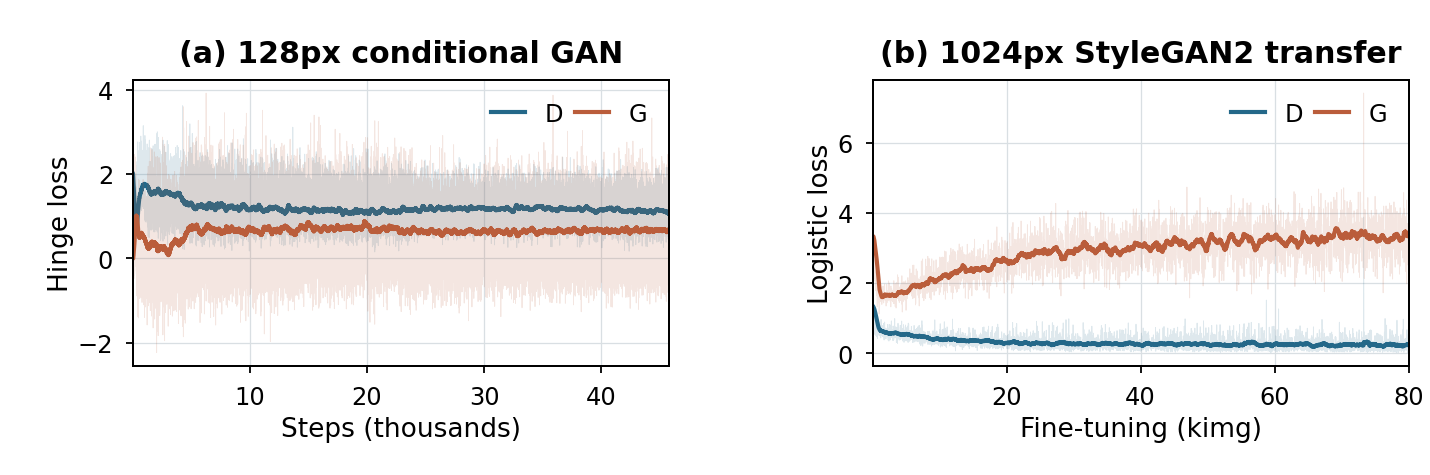
\includegraphics[width=.88\textwidth]{loss_curves.png}
\caption{Discriminator and generator losses for the complete scratch (left) and transfer (right) runs. Pale traces show updates; solid traces show moving averages (250 and 50 updates). Loss scales differ across objectives.}
\label{fig:losses}
\end{figure}

\section{Evaluation and results}
Each final evaluation uses 1,000 real and 1,000 generated images. PyTorch-Ignite~\cite{ignite} maps outputs to $[0,1]$, antialias-resizes to $299^2$, then applies ImageNet Inception-v3. Pool3 FID uses 2,048 features~\cite{heusel}; the tutorial-default FID uses class probabilities and a different scale. IS measures predicted-class concentration and diversity~\cite{salimans}. Transfer rows share test images, seed 32026, preprocessing, and truncation $\psi=1$.

\begin{table}[H]
\caption{Complete recorded 1,000-pair evaluations. Lower FID and higher IS are favorable. The independent GAN has a different split, conditioning, and resolution; its row is contextual rather than a like-for-like comparison.}
\label{tab:metrics}
\centering
\small
\begin{tabular}{@{}lrrr@{}}
\toprule
Model & Pool3 FID $\downarrow$ & Ignite FID $\downarrow$ & IS $\uparrow$ \\
\midrule
Independent GAN, epoch 40 & 177.32 & 0.1335 & 2.405 \\
Public StyleGAN2, 0 kimg & 55.97 & 0.0523 & 7.019 \\
Fine-tuned, 79.459 kimg & 58.12 & 0.0578 & 7.080 \\
\bottomrule
\end{tabular}
\end{table}

Relative to initialization, transfer changes test FID by $+2.15$ (worse) and IS by $+0.062$ (better). The separate 512-pair validation FID changes from 85.63 at 0 kimg to 87.51 at 80 kimg. These results do not show consistent fidelity improvement; much of the visual quality is already present in the public prior.

\begin{figure}[H]
\centering
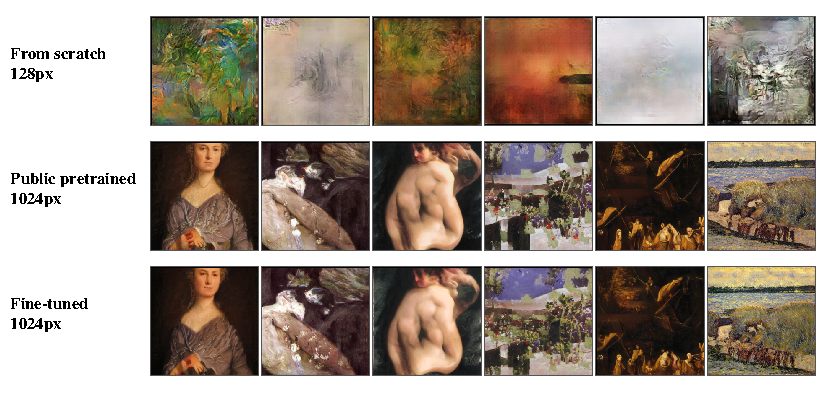
\includegraphics[width=\textwidth]{generated_examples.pdf}
\caption{Twenty-four fixed generated examples, eight per model. Top: independent $128^2$ GAN (grid positions 0, 9, 18, 27, 36, 45, 54, 63). Middle and bottom: public and selected fine-tuned StyleGAN2 with identical seeds 2026--2033 and $\psi=1$. Complete grids (64 scratch images and 16 per transfer checkpoint) are linked in the repository.}
\label{fig:examples}
\end{figure}

\section{Interpretation and limitations}
The scratch GAN learns painterly texture but weak long-range structure; transfer samples show sharper subjects. Different resolutions, conditioning, and splits prevent attributing their FID gap to any single factor. Public pretraining on WikiArt may overlap our test set, so transfer-test metrics do \emph{not} establish unseen-pretraining generalization. FID and IS are finite-sample, ImageNet-based estimates with known bias~\cite{chong}. A stronger study requires verified disjoint pretraining data, common-split ablations, and more test samples.

\clearpage
\begin{thebibliography}{11}
\raggedright
\bibitem{goodfellow} I.~Goodfellow et al. Generative Adversarial Nets. \emph{NeurIPS}, 2014. \url{https://proceedings.neurips.cc/paper/2014/hash/f033ed80deb0234979a61f95710dbe25-Abstract.html}.
\bibitem{wikiart} steubk. \emph{WikiArt} dataset, Kaggle. \url{https://www.kaggle.com/datasets/steubk/wikiart}.
\bibitem{miyatoProjection} T.~Miyato and M.~Koyama. cGANs with Projection Discriminator. \emph{ICLR}, 2018. \url{https://arxiv.org/abs/1802.05637}.
\bibitem{miyatoSpectral} T.~Miyato, T.~Kataoka, M.~Koyama, and Y.~Yoshida. Spectral Normalization for Generative Adversarial Networks. \emph{ICLR}, 2018. \url{https://openreview.net/forum?id=B1QRgziT-}.
\bibitem{karrasStylegan2} T.~Karras et al. Analyzing and Improving the Image Quality of StyleGAN. \emph{CVPR}, 2020. \url{https://openaccess.thecvf.com/content_CVPR_2020/html/Karras_Analyzing_and_Improving_the_Image_Quality_of_StyleGAN_CVPR_2020_paper.html}.
\bibitem{karrasADA} T.~Karras et al. Training Generative Adversarial Networks with Limited Data. \emph{NeurIPS}, 2020. \url{https://proceedings.neurips.cc/paper/2020/hash/8d30aa96e72440759f74bd2306c1fa3d-Abstract.html}.
\bibitem{baylies} P.~Baylies. \emph{WikiArt\_Uncond2}, public pretrained checkpoint. Internet Archive, 2020. \url{https://archive.org/details/wikiart-stylegan2-conditional-model}.
\bibitem{heusel} M.~Heusel et al. GANs Trained by a Two Time-Scale Update Rule Converge to a Local Nash Equilibrium. \emph{NeurIPS}, 2017. \url{https://proceedings.neurips.cc/paper/2017/hash/8a1d694707eb0fefe65871369074926d-Abstract.html}.
\bibitem{salimans} T.~Salimans et al. Improved Techniques for Training GANs. \emph{NeurIPS}, 2016. \url{https://proceedings.neurips.cc/paper/2016/hash/8a3363abe792db2d8761d6403605aeb7-Abstract.html}.
\bibitem{ignite} PyTorch-Ignite. GAN Evaluation: Fr\'echet Inception Distance and Inception Score. \url{https://pytorch-ignite.ai/blog/gan-evaluation-with-fid-and-is/}.
\bibitem{chong} M.~J. Chong and D.~Forsyth. Effectively Unbiased FID and Inception Score and Where to Find Them. \emph{CVPR}, 2020. \url{https://openaccess.thecvf.com/content_CVPR_2020/html/Chong_Effectively_Unbiased_FID_and_Inception_Score_and_Where_to_Find_CVPR_2020_paper.html}.
\end{thebibliography}

\end{document}
